\RequirePackage[l2tabu, orthodox]{nag}

\documentclass[11pt,a4paper,titlepage]{article}
\makeatletter
\def\@seccntformat#1{\llap{\csname the#1\endcsname\quad}}
\makeatother

\usepackage{mdframed}
\usepackage[table]{xcolor}
\usepackage{graphicx}
\usepackage[top=0.75in, bottom=0.75in, left=1in, right=0.75in]{geometry}
\usepackage{arcs}
\usepackage{covington}
\usepackage{dvgloss}
\usepackage{microtype}
\usepackage{tipa}
\let\ipa\textipa
\usepackage{vowel}
\usepackage{multicol}
\usepackage{needspace}
\usepackage{pdfpages}
\usepackage[colorlinks=true, linkcolor=black, urlcolor=cyan, pdfborder={0 0 0}]{hyperref}
\usepackage{fontspec}
\usepackage{gb4e}
\usepackage{setspace}
\usepackage{multirow}
\usepackage{changepage}
\usepackage{lipsum}
\usepackage{parskip}
\usepackage{changepage}
\DeclareUTFcharacter[\UTFencname]{x2329}{\textlangle}
\DeclareUTFcharacter[\UTFencname]{x232A}{\textrangle}
\DeclareUTFcharacter[\UTFencname]{x0335}{\strokeoverlay}
\newcommand\phoneme[1]{/\,#1\,/}
\newcommand\phone[1]{[\,#1\,]}
\newcommand\orth[1]{\textlangle\,#1\,\textrangle}
\newcommand\gstop{ʔ}
\newcommand\turnc{ɔ}
\newcommand\textlong{ː}
\newcommand\hightone{˥}
\newcommand\lowtone{˩}
\newcommand\midrising{˧˥}
\newcommand\midfalling{˧˩}
\newcommand\highfalling{˥˧}
\newcommand\lowrising{˩˧}
\newcommand{\BlankCell}{}
\newcommand\tl{ɬ}
\renewcommand\omega{ʊ}
\renewcommand\epsilon{ɛ}
\renewcommand\iota{ɪ}
\onehalfspace

\newmdenv[
  
]{example-box}

\renewenvironment{example}
{\vspace{\baselineskip}\begin{adjustwidth}{1em}{0pt}\begin{example-box}}
{\end{example-box}\end{adjustwidth}}

\newenvironment{original}
{\itshape}
{\upshape}

\newenvironment{translation}
{``}
{''}

\author{Benjamin Smith}
\title{Kiswóna Grammar}
\date{July 29, 2013}
\setmainfont{Charis SIL}

\begin{document}
	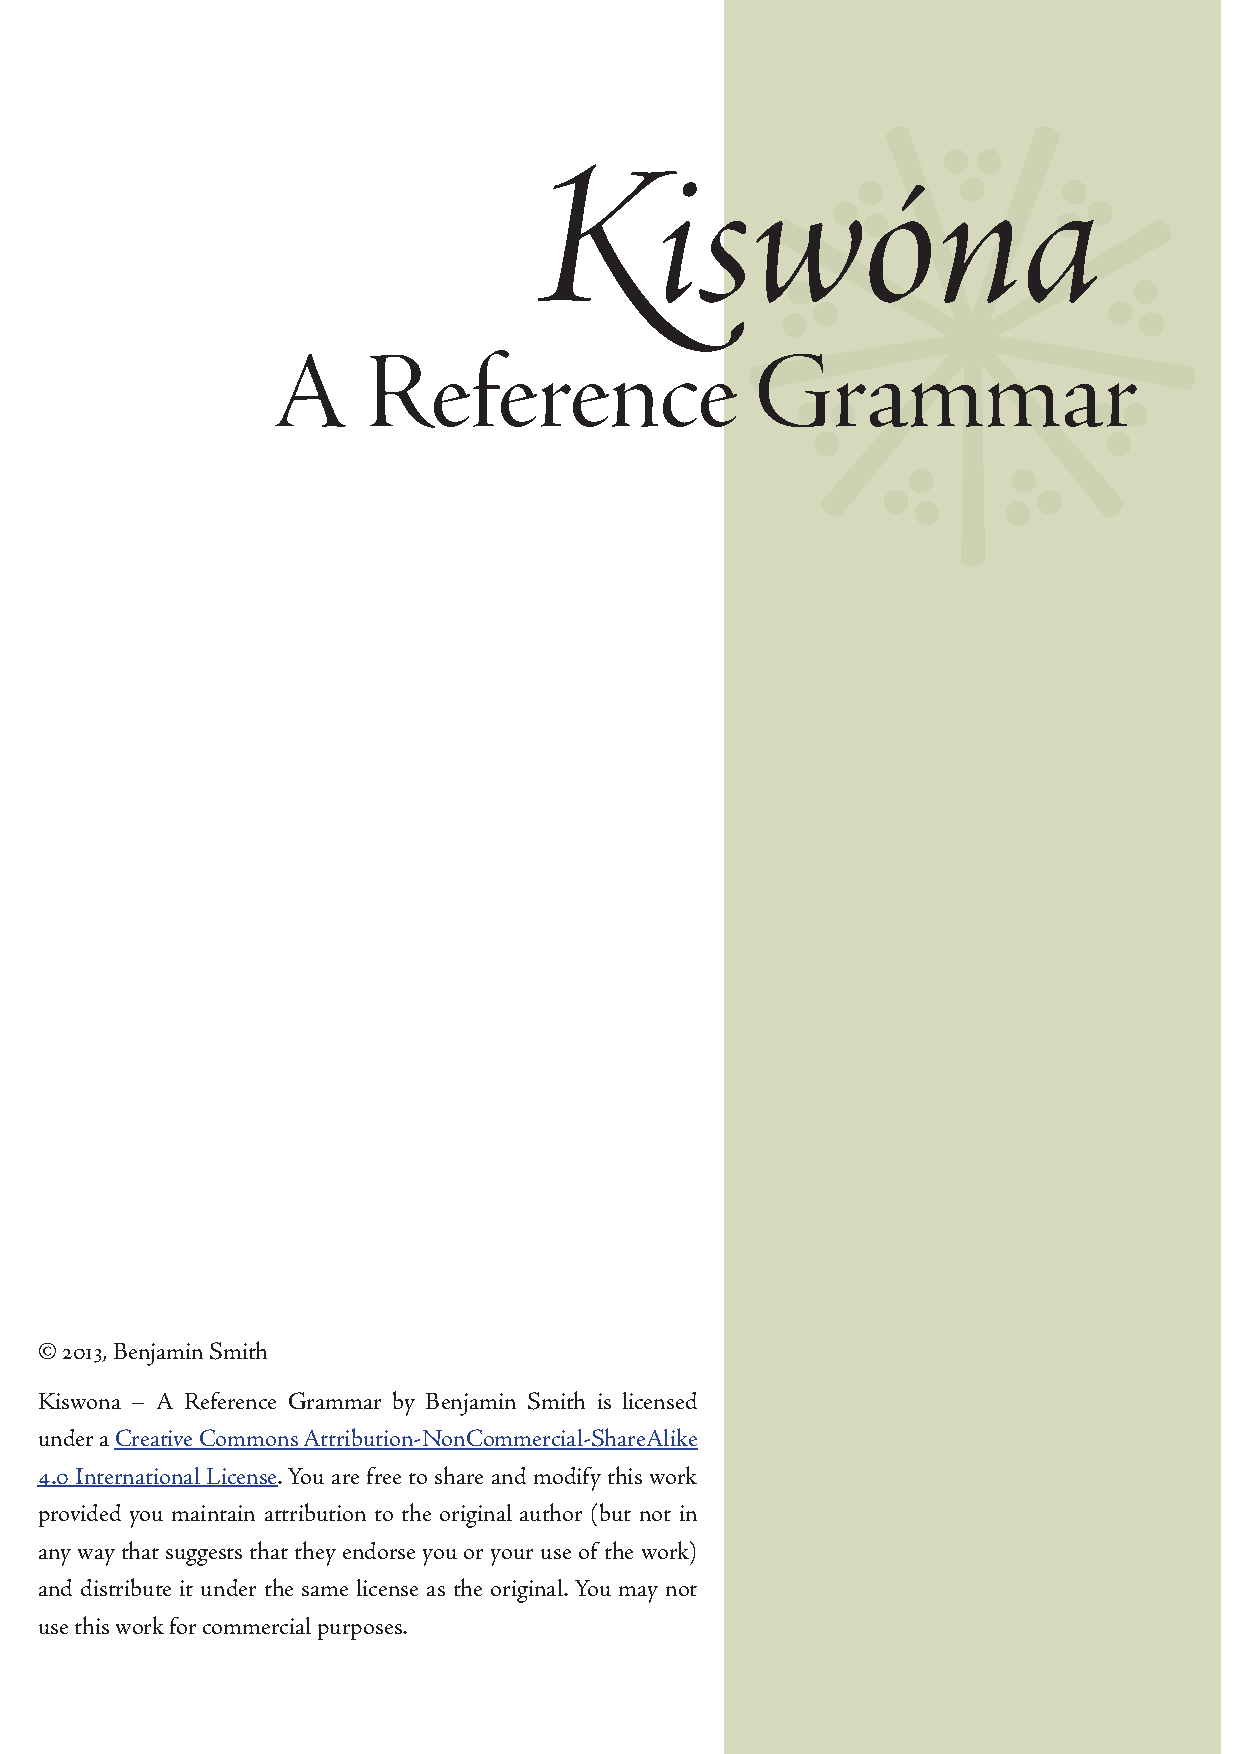
\includepdf[pages={1}]{cover.pdf}

	\tableofcontents

	\newpage

	\section{Introduction}
		Classical Kiswóna \phone{ki.zwo\hightone na} is the lingua franca and literary language of the nations of the Ondási. Inspiration for Kiswóna has been drawn from the Amerindian languages, particularly the Iroquoian and Athabascan languages. The Ondási nations are partially inspired by the Iroquois League.

	\section{Legend}
		\begin{tabular}{l l l l l l}
			1 & 1\textsuperscript{st} person & \textsc{exh} & exhortative & \textsc{obv} & obviative \\
			2 & 2\textsuperscript{nd} person & \textsc{gen} & genitive & \textsc{opt} & optative \\
			3 & 3\textsuperscript{rd} person & \textsc{gno} & gnomic & \textsc{per} & perlative \\
			\textsc{abl} & ablative & \textsc{hab} & habitual & \textsc{pfv} & perfective \\
			\textsc{ade} & adessive & \textsc{ill} & illative & \textsc{pl} & plural \\
			\textsc{all} & allative & \textsc{imp} & imperative & \textsc{prs} & present \\
			\textsc{ass} & assumptive & \textsc{inch} & inchoative & \textsc{rec} & reciprocal \\
			\textsc{att} & attenuative & \textsc{incl} & inclusive & \textsc{refl} & reflexive \\
			\textsc{bene} & benefactive & \textsc{ine} & inessive & \textsc{rel} & relativizer \\
			\textsc{c} & complementizer & \textsc{infr} & inferential & \textsc{rfut} & remote future \\
			\textsc{caus} & causative & \textsc{inh} & inhortative & \textsc{rpst} & remote past \\
			\textsc{cess} & cessative & \textsc{inst} & instrumental & \textsc{subj} & subjunctive \\
			\textsc{com} & comitative & \textsc{int} & intensive & \textsc{sub} & subessive \\
			\textsc{cond} & conditional & \textsc{ipfv]} & imperfective & \textsc{sup} & superessive \\
			\textsc{ded} & deductive & \textsc{nec} & necessitative & \textsc{svl} & semi-volitional \\
			\textsc{du} & dual & \textsc{neg} & negative & \textsc{voc} & vocative \\
			\textsc{dub} & dubitative & \textsc{nfut} & near future & \textsc{vol} & volitional \\
			\textsc{ela} & elative & \textsc{npst} & near past & & \\
			\textsc{excl} & exclusive & \textsc{nvl} & non-volitional & & \\
		\end{tabular}

	\section{Phonology}

		\subsection{Phoneme Inventory}
			Kisw\'ona features seventeen consonants and either five or ten vowels, depending on how it is analyzed. It is notable for its complete lack of bilabial and rhotic consonants, having lost the bilabial nasal [m], voiced bilabial fricative [β], retroflex approximant [ɻ] and alveolar trill [r] present in the Boreal and Occidental as well as Proto–Kanneyan languages.		

			\subsubsection{Consonants}

				\paragraph{Nasals} ~\\
					Kisw\'ona has a single nasal consonant, \phoneme{n}.

				\paragraph{Stops} ~\\
					Five stops are contrasted, \phoneme{t d k g \gstop}. The glottal stop is represented by \orth{q}.

				\paragraph{Fricatives} ~\\
					Kisw\'ona has five fricatives \phoneme{s \esh{} \c{c} x \tl} represented by \orth{s x hy h tl}.
				\paragraph{Approximants} ~\\
					There are three approximants \phoneme{\textturnw{} w j} represented by \orth{hw w y}.

				\paragraph{Affricates} ~\\
					Kisw\'ona has two affricates \phoneme{\t{ts} \t{t\esh}} represented by \orth{ts c}.

			\subsubsection{Vowels}
				Kisw\'ona has five base vowels \phoneme{i u e o a} with contrastive length, tone and nasalization. Nasalization is marked with ogonki and length is indicated by doubling of vowels.

    \subsection{Allophony}
      \subsubsection{Consonants}
        The alveolar stops \phoneme{t d} exist in free variation with their dental counterparts \phone{\textipa{\textsubbridge{t} \textsubbridge{d}}}. When the alveolar nasal precedes a dental stop it too becomes dental \phone{\textipa{\textsubbridge{n}}}.

        When a fricative occurs intervocally or between a vowel and a voiced consonant, it becomes voiced yielding \phone{z \textipa{Z J G \textlyoghlig}}.

        \begin{example}
          \begin{original}
            Test
          \end{original}

          \begin{translation}
            Test
          \end{translation}
        \end{example}

        Adjacent fricatives undergo regressive assimilation. \phoneme{\c{c}\esh{}} is realised as \phone{\esh{}\textlong}. These changes are not reflected in the orthography.

      \subsubsection{Vowels}
        When vowels are nasalized their quality changes.
				\vspace{10pt}

				\begin{tabular}{|l|c|c|c|c|c|}
					\hline
					\textbf{Bare}  & a \phone{a} & e \phone{e} & i \phone{i} & o \phone{o} & u \phone{u} \\
					\hline
					\textbf{Nasal} & \k{a} \phone{\~\ae} & \k{e} \phone{\~\epsilon} & \k{i} \phone{\~\iota} & \k{o} \phone{\~\turnc} & \k{u} \phone{\~\omega} \\
					\hline
				\end{tabular}

		\subsection{Phonotactics}
			\subsubsection{Syllable Structure}
				The basic structure of the Kisw\'ona syllable is (C)(C)V(C). The following constraints exist:
				\begin{itemize}
					\item{Hiatus is restricted.}
				\end{itemize}
		\subsection{Tone}
			\lipsum[1]
	\section{Animacy}
		\lipsum[1]
	\section{Verbs, Adjectives and Adverbs}
		\lipsum[1]
		\subsection{Verb Morphology}
			\lipsum[1]
			\subsubsection{Tense}
				\lipsum[1]
			\subsubsection{Aspect}
				\lipsum[1]
			\subsubsection{Mood}
				\lipsum[1]
			\subsubsection{Voice}
				\lipsum[1]
		\subsection{Transitivity}
			\lipsum[1]
		\subsection{Adjectives}
			\lipsum[1]
		\subsection{Adverbs}
			\lipsum[1]
	\section{Nouns}
		\lipsum[1]
		\subsection{Number}
			\lipsum[1]
		\subsection{Case}
			\lipsum[1]
	\section{Postpositions}
		\lipsum[1]
	\section{Interrogatives}
		\lipsum[1]
		\subsection{Polar Questions}
			\lipsum[1]
		\subsection{Tag Questions}
		\subsection{Wh-qestions}
	\section{Anaphora}
		\subsection{Personal Pronouns}
		\subsection{Classifiers}
		\subsection{Correlatives}
			\begin{adjustwidth}{-1in}{-0.75in}
				\begin{center}
					\scriptsize
					\begin{tabular}{|c c| c c c c c c c c c|}
						\hline
						\rowcolor[gray]{0.8}\multicolumn{2}{|c}{} && \multicolumn{3}{c}{\textbf{Demonstrative}} & \multicolumn{5}{c|}{\textbf{Quantifier}} \\ \cline{4-11}
						\rowcolor[gray]{0.8}\multicolumn{2}{|c}{} &\multirow{-2}{*}{\textbf{Interrogative}} & \textbf{Proximal} & \textbf{Medial} & \textbf{Distal} & \textbf{Existential} & \textbf{Elective} & \textbf{Universal} & \textbf{Negatory} & \textbf{Alternative} \\
						\hline
						\multicolumn{2}{|c|}{\cellcolor[gray]{0.8}\textbf{Determiner}} & éétla & éé & egáá & egaa & enlé & déé & enne & tséé & egke \\
						\cellcolor[gray]{0.8} & \cellcolor[gray]{0.8} \textbf{Animate} & tlaka & aka & káá & akaa & angla & daka & enke & tsaka & agka \\
						\cellcolor[gray]{0.8} & \cellcolor[gray]{0.8} \textbf{Inanimate} & éétla & éé & egáá & egaa & enlé & déé & enne & tséé & egke \\
						\cellcolor[gray]{0.8} & \cellcolor[gray]{0.8} \textbf{Out of Two} & kítla & kíí & ekíí & ekii & inkli & gíí & inkí & tsikí & igkí \\
						\multirow{-4}{*}{\cellcolor[gray]{0.8}\textbf{Pronoun}} & \cellcolor[gray]{0.8} \textbf{Out of Many} & sítla & síí & esíí & esii & inxí & síí & insí & tsíí & iski \\
						\hline
						\cellcolor[gray]{0.8} & \cellcolor[gray]{0.8} \textbf{Location} & lá & élá & alá & láá & anlá & ilá & telá & tselá & lágká \\ 
						\cellcolor[gray]{0.8} & \cellcolor[gray]{0.8} \textbf{Source} & tláka & éláka & aláka & lááka & anláka & iláka & teláka & tseláka & lágkáka \\
						\cellcolor[gray]{0.8} & \cellcolor[gray]{0.8} \textbf{Goal} & tláku & éláku & aláku & lááku & anláku & iláku & teláku & tseláku & lágkáku \\
						\cellcolor[gray]{0.8} & \cellcolor[gray]{0.8} \textbf{Time} & tselé & allé & lé & lé & enlé & illé & tellé & tsellé & légké \\
						\cellcolor[gray]{0.8} & \cellcolor[gray]{0.8} \textbf{Manner} & éégistla & éégis & egáágis & egaagis & enlégis & déégis & ennegis & tséégis & egkegis \\
						\multirow{-6}{*}{\cellcolor[gray]{0.8} \textbf{Pro-adverb}} & \cellcolor[gray]{0.8} \textbf{Reason} & hyotla & hyo & ehyóó & ehyoo & ontlo & hyo & onhyo & thyo & hyogko \\
						\hline
					\end{tabular}
				\end{center}
			\end{adjustwidth}
	\section{Conjunctions}
		\lipsum[1]
	\section{Syntax}
		\lipsum[1]
	\section{Derivational Morphology}
		\lipsum[1]
	\section{Numbers}
		\lipsum[1]
	\section{Example Texts}
		\subsection{The Babel Text}
			\textsuperscript{1}Téluhyex Tséqako kiséwatl aníhwe ankáte.
			\textsuperscript{2}Khwotsáka axwegénlete \'atle, itletl xínay\`a axiy\'aneta, lááy\`a axtsáwiteqa técata le.
			\textsuperscript{3}«Dixluusàyaxíquke nlakaásitl dixcúqįkequqa.» axlakáta le. Dúwotl luusàt axankáte xoxóksin cat axankáteqa.
			\textsuperscript{4}«Tséqaso tsedixdíyudénda issé axtloheyaxíkeqa le.» axlakátan le. «Sihwáku otlxanánde na ksindótl cúgwitla dixyaxíkeqa.»
			\textsuperscript{5}Ksindótl cúgwitla oxhayanete issé Sáswax ngosita le.
			\textsuperscript{6}«Ixásoqa! Ondásin aníhwe naquyéqe, kiséwatl aníhwe axankáqe, éétl axyaxíqu otl axhyinláqa na tséétl lídodinde.» Sáswax lakáta le.
			\textsuperscript{7}«Kiséwasitl ako dixkádaqa issé dixngosikeqa. Kiséwasitl ako tsewotúnden le.»
			\textsuperscript{8}Sáswax Tséqaso andíyudéta cúgwin axyaxítula le.
			\textsuperscript{9}Sáswax lááye kiséwasitl téluhye Tséqako kádata tsáagi, dádeletl ontlohéqa ehyóó. Sáswax lááka Tséqaso andíyudéta.
			\\~

			\gl{téluhye-x Tséqa-ko kiséwa-tl aníhwe anká-t-e}{entirety-\textsc{a} Ts\'eqa-\textsc{gen} tongue-\textsc{obl} one use-\textsc{fpst}-\textsc{ipfv}}

			\vspace{12pt}
			\gl{khwotsá-ka a-x-wegénle-t-e \'atle}{east-\textsc{abl} 3.\textsc{pl}-\textsc{a}-travel-\textsc{fpst}-\textsc{ipfv} while}

			\vspace{12pt}
			\gl{itle-n xína-y\`a a-x-iy\'ane-t-a}{plain-\textsc{obl} Shinar-\textsc{ine} 3.\textsc{pl}-\textsc{a}-stumble.upon-\textsc{fpst}-\textsc{ipfv}}

			\vspace{12pt}
			\gl{láá-y\`a a-x-tsáwi-t-e=a téca-t-a le}{there.\textsc{dist}-\textsc{ine} 3.\textsc{pl}-\textsc{a}-dwell-\textsc{fpst}-\textsc{pfv}=and happen-\textsc{fpst}-\textsc{pfv} then}
\end{document}
